\section{La programmation orientée Objet}
\begin{frame}
	\begin{center}
	\huge
	La programmation Orientée Objet
	\end{center}
\end{frame}

\subsection{Notion d'objet} %%%%%%%%%%%%%%%%%%%%%%%%%%%%%%%%%%%%%%%%%
\begin{frame}
	\frametitle{Comme une boite}
	\begin{center}
	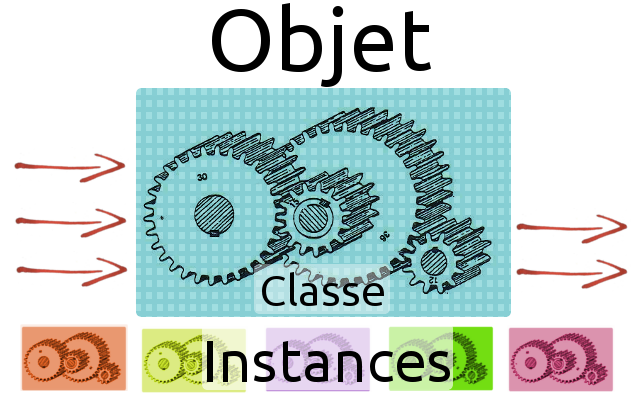
\includegraphics[width=9cm]{pics/explObj1.png}
	\end{center}
\end{frame}
\begin{frame}
	\frametitle{Attributs/Méthodes}
	\begin{center}
	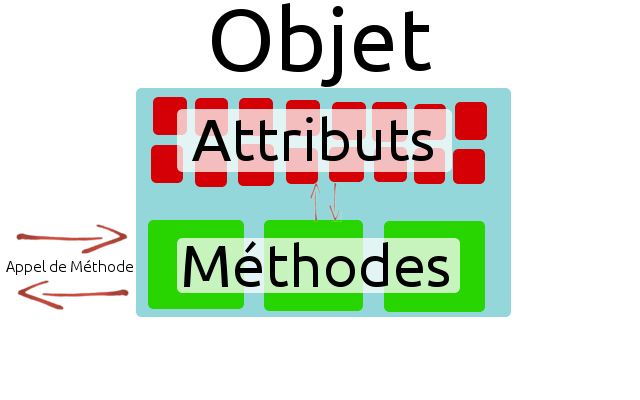
\includegraphics[width=9cm]{pics/explObj2.png}
	\end{center}
\end{frame}
\begin{frame}[fragile]
	\frametitle{Création d'instance et appel de fonction}
	\begin{lstlisting}
let (c1,c2) =
  let m1 = new CoffeMachine(Bresile)
  and m2 = new CoffeMachine(Islande)
  in let _ = 
    m1#addWater(1000);
    m2#addWater(42000)
  in let _ =
    m1#headUp();
    m2#headUp()
  in (m1#getCoffe(1),m2#getCoffe(3))
;;
	\end{lstlisting}
\end{frame}

\subsection{La déclaration d'un objet} %%%%%%%%%%%%%%%%%%%%%%%%%%%%%%
\begin{frame}[fragile]
	\frametitle{Syntaxe}
	\begin{lstlisting}
class name pa1..pan =
  object
    (*Attributs*)
    
    (*Methods*)
  end
;;
	\end{lstlisting}
\end{frame}

\begin{frame}[fragile]
	\frametitle{Déclaration d'attribut}
	\textit{Respectez le typage}\\
	\textbf{Simple}
	\begin{lstlisting}
  val name = expr
	\end{lstlisting}
	\textbf{Modifiable}
	\begin{lstlisting}
  val mutable name = expr
  name <- expr
	\end{lstlisting}
	\textbf{Lorsque rien ne marche : Le type Option}
	\begin{lstlisting}
  val mutable name = None
  name <- Some expr
	\end{lstlisting}
\end{frame}

\begin{frame}[fragile]
	\frametitle{Déclaration de méthode}
	\textbf{simple}
	\begin{lstlisting}
  method name p1 ...pn = expr
	\end{lstlisting}
	\textbf{privée}\\
	\begin{minipage}{0.4\textwidth}
  	\begin{lstlisting}
  class ... =
    object
    ...
    end
		\end{lstlisting}
	\end{minipage}$\Rightarrow$
	\begin{minipage}{0.4\textwidth}
		\begin{lstlisting}
  class ... =
    object (self)
    ...
    end
		\end{lstlisting}
	\end{minipage}
	\begin{lstlisting}
  method private name p1 ...pn = expr
  self#privateMethod ...
	\end{lstlisting}
\end{frame}

\begin{frame}[fragile]
	\frametitle{Initialisation}
	\begin{lstlisting}
  class ... =
    object (self)
    
    (*Attributs*)
    
    initializer
      expr
    
    (*Methods*)
    end
	\end{lstlisting}
\end{frame}

\begin{frame}
	\frametitle{Attributs polymorphiques}
	
\end{frame}

\subsection{L'heritage} %%%%%%%%%%%%%%%%%%%%%%%%%%%%%%%%%%%%%%%%%%%%%
\begin{frame}

\end{frame}

\subsection{Le polymorphisme d'inclusion} %%%%%%%%%%%%%%%%%%%%%%%%%%%
\begin{frame}

\end{frame}
